\documentclass{article} 
\usepackage{tikz}
\usepackage{xcolor}
\usetikzlibrary{matrix}
\usetikzlibrary{arrows} % additional arrows
\usetikzlibrary{shapes,snakes}

\begin{document}



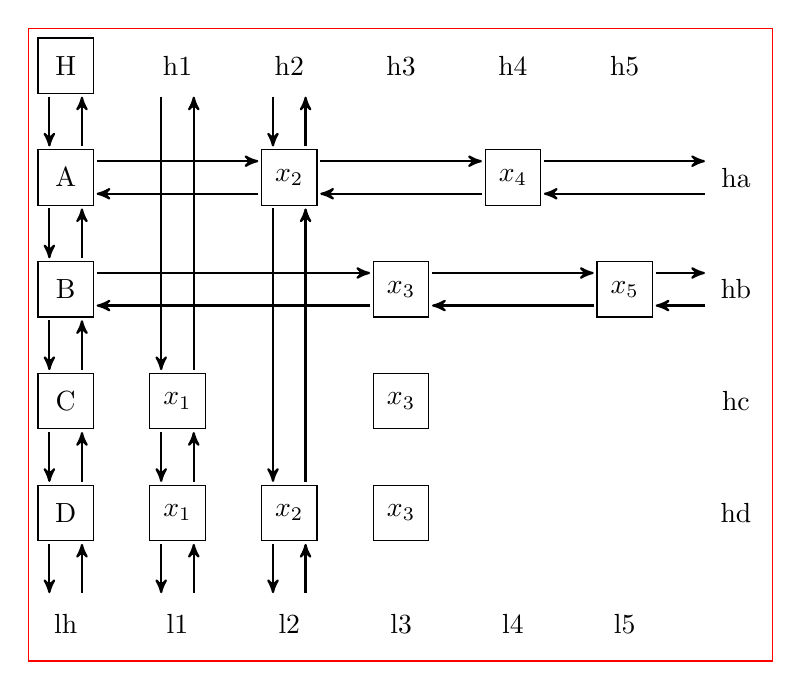
\begin{tikzpicture}
[
every node/.style={
	row sep=2em, 
	column sep=2em, 
	minimum height=2em,
	minimum width=2em,
	draw=black,
	rectangle},
regArr/.style={
	->,
	>=stealth',
    thick,
    shorten <=1pt,
    shorten >=1pt,}
]
\matrix [draw=red]
{
\node (h) {H}; & \node[draw=none] (h1) {h1}; & \node[draw=none] (h2) {h2}; & \node[draw=none] (h3) {h3}; & \node[draw=none] (h4) {h4}; & \node[draw=none] (h5) {h5}; & \\

\node (ra) {A}; &  & \node (a2) {$x_2$}; & & \node (a4) {$x_4$}; & &\node[draw=none] (ha) {ha};\\
\node (rb) {B}; &  &  & \node (b3) {$x_3$}; & & \node (b5) {$x_5$}; & \node[draw=none] (hb) {hb};\\
\node (rc) {C}; & \node (c1) {$x_1$}; & & \node (c3) {$x_3$}; & &  & \node[draw=none] (hc) {hc};\\
\node (rd) {D}; & \node (d1) {$x_1$}; & \node (d2) {$x_2$}; & \node (d3) {$x_3$}; & & & \node[draw=none] (hd) {hd};\\
\node[draw=none] (lh) {lh}; & \node[draw=none] (l1) {l1}; & \node[draw=none] (l2) {l2}; & \node[draw=none] (l3) {l3}; & \node[draw=none] (l4) {l4}; & \node[draw=none] (l5) {l5}; & \\
};

%degree location of arrow anchor 
\def\bo{240} %bottom, going out
\def\bi{300} %bottom, going in
\def\to{60} %top, going out
\def\ti{120} %top, going in

\def\ro{30} %right, going out
\def\ri{330} %right, going in
\def\lo{210} %left, going out
\def\li{150} %left, going in

%header column
\draw [regArr] (h.\bo) -- (ra.\ti);
\draw [regArr] (ra.\to) -- (h.\bi);
\draw [regArr] (ra.\bo) -- (rb.\ti);
\draw [regArr] (rb.\to) -- (ra.\bi);
\draw [regArr] (rb.\bo) -- (rc.\ti);
\draw [regArr] (rc.\to) -- (rb.\bi);
\draw [regArr] (rc.\bo) -- (rd.\ti);
\draw [regArr] (rd.\to) -- (rc.\bi);
\draw [regArr] (rd.\bo) -- (lh.\ti);
\draw [regArr] (lh.\to) -- (rd.\bi);

%x_1 column
\draw [regArr] (h1.\bo) -- (c1.\ti);
\draw [regArr] (c1.\to) -- (h1.\bi);
\draw [regArr] (c1.\bo) -- (d1.\ti);
\draw [regArr] (d1.\to) -- (c1.\bi);
\draw [regArr] (d1.\bo) -- (l1.\ti);
\draw [regArr] (l1.\to) -- (d1.\bi);

%x_2 column
\draw [regArr] (h2.\bo) -- (a2.\ti);
\draw [regArr] (a2.\to) -- (h2.\bi);
\draw [regArr] (a2.\bo) -- (d2.\ti);
\draw [regArr] (d2.\to) -- (a2.\bi);
\draw [regArr] (d2.\bo) -- (l2.\ti);
\draw [regArr] (l2.\to) -- (d2.\bi);

%A row
\draw [regArr] (ra.\ro) -- (a2.\li);
\draw [regArr] (a2.\lo) -- (ra.\ri);
\draw [regArr] (a2.\ro) -- (a4.\li);
\draw [regArr] (a4.\lo) -- (a2.\ri);
\draw [regArr] (a4.\ro) -- (ha.\li);
\draw [regArr] (ha.\lo) -- (a4.\ri);

%B row
\draw [regArr] (rb.\ro) -- (b3.\li);
\draw [regArr] (b3.\lo) -- (rb.\ri);
\draw [regArr] (b3.\ro) -- (b5.\li);
\draw [regArr] (b5.\lo) -- (b3.\ri);
\draw [regArr] (b5.\ro) -- (hb.\li);
\draw [regArr] (hb.\lo) -- (b5.\ri);

%\draw [regArr] (rb.\ro) to [bend left=10] (b5.\li);

 
\end{tikzpicture}




\end{document}